% DataSynth Executive Overview
% Compile with: pdflatex datasynth-executive-overview.tex (run twice for TOC)
\documentclass[11pt,a4paper]{article}

% ── Packages ──────────────────────────────────────────────────────────────────
\usepackage[utf8]{inputenc}
\usepackage[T1]{fontenc}
\usepackage{lmodern}
\usepackage[margin=2.4cm]{geometry}
\usepackage{graphicx}
\usepackage{xcolor}
\usepackage{titlesec}
\usepackage{enumitem}
\usepackage{booktabs}
\usepackage{tabularx}
\usepackage{multirow}
\usepackage{fancyhdr}
\usepackage{hyperref}
% fontawesome5 removed — using text symbols instead
\usepackage{tcolorbox}
\usepackage{tikz}
\usepackage{pgfplots}
\usepackage{amssymb}
\pgfplotsset{compat=1.18}
\usetikzlibrary{arrows.meta, positioning, calc, shapes.geometric, backgrounds, fit}

% ── Colours ───────────────────────────────────────────────────────────────────
\definecolor{brand}{HTML}{1A2744}      % Deep navy
\definecolor{accent}{HTML}{2E86AB}     % Teal blue
\definecolor{highlight}{HTML}{F18F01}  % Amber
\definecolor{success}{HTML}{2D936C}    % Green
\definecolor{lightbg}{HTML}{F5F7FA}    % Light background
\definecolor{midgray}{HTML}{6C757D}    % Muted text

% ── Heading styles ────────────────────────────────────────────────────────────
\titleformat{\section}
  {\Large\bfseries\color{brand}}
  {\thesection}{1em}{}[\vspace{-0.4em}\textcolor{accent}{\rule{\textwidth}{1.2pt}}]

\titleformat{\subsection}
  {\large\bfseries\color{brand}}
  {\thesubsection}{0.8em}{}

\titleformat{\subsubsection}
  {\normalsize\bfseries\color{accent}}
  {\thesubsubsection}{0.6em}{}

% ── Header / Footer ──────────────────────────────────────────────────────────
\pagestyle{fancy}
\fancyhf{}
\renewcommand{\headrulewidth}{0.4pt}
\fancyhead[L]{\small\textcolor{midgray}{DataSynth --- Executive Overview}}
\fancyhead[R]{\small\textcolor{midgray}{v0.2.3}}
\fancyfoot[C]{\small\textcolor{midgray}{\thepage}}

% ── Custom boxes ──────────────────────────────────────────────────────────────
\tcbset{
  keybox/.style={
    colback=lightbg, colframe=accent, boxrule=0.6pt,
    arc=3pt, left=8pt, right=8pt, top=6pt, bottom=6pt,
    fonttitle=\bfseries\color{brand}, title=#1
  },
  statbox/.style={
    colback=white, colframe=brand, boxrule=0.8pt,
    arc=4pt, left=6pt, right=6pt, top=4pt, bottom=4pt,
    width=0.30\textwidth
  }
}

% ── Hyperref setup ────────────────────────────────────────────────────────────
\hypersetup{
  colorlinks=true,
  linkcolor=brand,
  urlcolor=accent,
  citecolor=brand,
  pdftitle={DataSynth -- Enterprise Synthetic Data Platform},
  pdfauthor={DataSynth},
  pdfsubject={Executive Overview},
}

% ══════════════════════════════════════════════════════════════════════════════
\begin{document}

% ── Title page ────────────────────────────────────────────────────────────────
\begin{titlepage}
\begin{tikzpicture}[remember picture, overlay]
  % Background gradient bar
  \fill[brand] (current page.north west) rectangle
    ([yshift=-9cm]current page.north east);
  % Accent stripe
  \fill[accent] ([yshift=-9cm]current page.north west) rectangle
    ([yshift=-9.4cm]current page.north east);
  % Decorative dots
  \foreach \x in {0.5,1.0,...,5.0} {
    \foreach \y in {0.5,1.0,...,3.0} {
      \fill[white, opacity=0.04] ([xshift=\x cm, yshift=-\y cm]current page.north west)
        circle (1.5pt);
    }
  }
\end{tikzpicture}

\vspace*{1.5cm}
\begin{flushleft}
  {\fontsize{38}{44}\selectfont\bfseries\textcolor{white}{DataSynth}}\\[0.5em]
  {\fontsize{16}{20}\selectfont\textcolor{white!85}{Enterprise Synthetic Data Platform}}\\[0.3em]
  {\large\textcolor{white!65}{High-Performance Generation for Accounting, Audit \& ML}}\\[0.3em]
  {\normalsize\textcolor{white!50}{Rust core \textbullet{} Python wrapper \textbullet{} REST/gRPC API \textbullet{} Desktop UI}}
\end{flushleft}

\vspace{5.5cm}

\begin{flushleft}
  \textcolor{midgray}{\large Executive Overview}\\[0.8em]
  {\Large\textcolor{brand}{\textbf{Version 0.2.3}}}\\[1.5em]
  \textcolor{midgray}{%
    Deterministic, privacy-preserving synthetic data generation\\
    for enterprise finance, compliance testing, and machine learning.%
  }
\end{flushleft}

\vfill
\begin{flushleft}
  \textcolor{midgray}{\small
    Built with Rust \& Python \textbullet{} 16 modular crates \textbullet{} 100\,K+ entries/sec\\[4pt]
    Open-source (Apache-2.0) \textbullet{} Commercial license available\\[4pt]
    \textbf{Contact:} \href{mailto:michael.ivertowski@ch.ey.com}{michael.ivertowski@ch.ey.com}
  }
\end{flushleft}
\end{titlepage}

% ── Table of Contents ─────────────────────────────────────────────────────────
\tableofcontents
\newpage

% ══════════════════════════════════════════════════════════════════════════════
\section{Executive Summary}

DataSynth is a high-performance synthetic data platform purpose-built for
enterprise accounting, audit analytics, and machine learning. Written in Rust
for maximum throughput and memory safety --- with a full Python wrapper for
data-science workflows --- it generates realistic, internally coherent
financial data that satisfies the statistical and structural properties of
real-world enterprise resource planning (ERP) systems.

\begin{tcolorbox}[keybox={Why DataSynth?}]
\begin{itemize}[leftmargin=1.2em, itemsep=3pt]
  \item \textbf{No real data required} --- eliminates privacy, regulatory, and
        procurement barriers to analytics development.
  \item \textbf{Full auditability} --- deterministic, seeded generation means
        every dataset is perfectly reproducible.
  \item \textbf{ML-ready from day one} --- ground-truth labels for fraud,
        anomalies, and data quality ship alongside every record.
  \item \textbf{Domain depth} --- covers the full accounting lifecycle:
        journal entries, document flows, subledgers, FX, intercompany,
        period close, and banking/AML.
  \item \textbf{Empirically grounded} --- statistical distributions for
        journal entry line items, amount patterns, and temporal volumes are
        calibrated against empirical research conducted on real-world
        enterprise datasets, ensuring synthetic output mirrors the
        structural properties of production ERP data.
\end{itemize}
\end{tcolorbox}

\subsection{At a Glance}

\vspace{0.6em}
\begin{center}
\begin{tabular}{@{}c@{\hspace{1.8em}}c@{\hspace{1.8em}}c@{}}
% Row 1
\begin{tcolorbox}[statbox, width=4.8cm]
  \centering
  {\fontsize{26}{30}\selectfont\bfseries\textcolor{accent}{100\,K+}}\\[3pt]
  {\small entries/sec (single thread)}
\end{tcolorbox} &
\begin{tcolorbox}[statbox, width=4.8cm]
  \centering
  {\fontsize{26}{30}\selectfont\bfseries\textcolor{accent}{20+}}\\[3pt]
  {\small labeled fraud typologies}
\end{tcolorbox} &
\begin{tcolorbox}[statbox, width=4.8cm]
  \centering
  {\fontsize{26}{30}\selectfont\bfseries\textcolor{accent}{10}}\\[3pt]
  {\small industry presets}
\end{tcolorbox} \\[0.8em]
% Row 2
\begin{tcolorbox}[statbox, width=4.8cm]
  \centering
  {\fontsize{26}{30}\selectfont\bfseries\textcolor{accent}{16}}\\[3pt]
  {\small modular Rust crates}
\end{tcolorbox} &
\begin{tcolorbox}[statbox, width=4.8cm]
  \centering
  {\fontsize{26}{30}\selectfont\bfseries\textcolor{accent}{14}}\\[3pt]
  {\small phases fully completed}
\end{tcolorbox} &
\begin{tcolorbox}[statbox, width=4.8cm]
  \centering
  {\fontsize{26}{30}\selectfont\bfseries\textcolor{accent}{4}}\\[3pt]
  {\small privacy levels}
\end{tcolorbox}
\end{tabular}
\end{center}

% ══════════════════════════════════════════════════════════════════════════════
\newpage
\section{Platform Capabilities}

\subsection{Enterprise Accounting Simulation}

DataSynth generates a complete, internally consistent accounting universe:

\begin{table}[h!]
\centering
\renewcommand{\arraystretch}{1.25}
\begin{tabularx}{\textwidth}{>{\bfseries\color{brand}}l X}
\toprule
\textbf{Domain} & \textbf{Capabilities} \\
\midrule
Journal Entries &
  Balanced debits/credits, Benford-compliant amounts, configurable line-item
  distributions, SAP ACDOCA format export. \\
Master Data &
  Vendors, customers, materials, fixed assets, employees with hierarchies,
  payment terms, credit ratings, and intercompany flags. \\
Document Flows &
  Full Procure-to-Pay (PO\,$\to$\,GR\,$\to$\,Invoice\,$\to$\,Payment) and
  Order-to-Cash (SO\,$\to$\,Delivery\,$\to$\,Invoice\,$\to$\,Receipt) with
  three-way match validation. \\
Intercompany &
  Matched IC journal entry pairs, transfer pricing (Cost-Plus, Resale-Minus,
  CUP), and consolidation elimination entries. \\
Subledgers &
  AR/AP open items and aging, fixed asset register with depreciation schedules,
  inventory positions and movements, GL-to-subledger reconciliation. \\
FX \& Translation &
  Ornstein--Uhlenbeck exchange rate process, multi-currency trial balance
  translation, currency translation adjustment entries. \\
Period Close &
  Month-end accruals, depreciation runs, year-end closing entries, fiscal
  period status tracking. \\
\bottomrule
\end{tabularx}
\end{table}

\subsection{Banking, KYC \& AML}

A dedicated banking module generates realistic transaction data for
anti-money-laundering testing:

\begin{itemize}[leftmargin=1.4em, itemsep=2pt]
  \item \textbf{Customer personas}: Retail, Business, Trust profiles with
        full KYC envelopes (declared turnover, source of funds, geographic
        exposure, cash intensity).
  \item \textbf{AML typologies}: Structuring, funnel accounts, layering
        schemes, money mule networks, round-tripping, and adversarial
        spoofing for robustness testing.
  \item \textbf{Ground-truth labels}: Entity-level risk classifications,
        transaction-level labels, and investigation narratives.
\end{itemize}

\subsection{Audit Simulation}

Generates ISA-compliant audit artifacts:

\begin{itemize}[leftmargin=1.4em, itemsep=2pt]
  \item Engagement metadata with materiality thresholds (ISA 320).
  \item Workpapers per ISA 230, evidence per ISA 500.
  \item Risk assessments (ISA 315/330), findings (ISA 265), and
        professional judgment documentation (ISA 200).
\end{itemize}

\subsection{COSO 2013 Internal Control Framework}

Full integration with the COSO Internal Control-Integrated Framework:

\begin{itemize}[leftmargin=1.4em, itemsep=2pt]
  \item \textbf{5 Components}: Control Environment, Risk Assessment,
        Control Activities, Information \& Communication, Monitoring Activities.
  \item \textbf{17 Principles}: Complete principle coverage with control mappings.
  \item \textbf{Control Scopes}: Entity-level, transaction-level, IT general,
        and IT application controls.
  \item \textbf{Maturity Levels}: 6-level model (Non-Existent through Optimized).
  \item \textbf{Export}: \texttt{coso\_control\_mapping.csv} with principle-level granularity.
\end{itemize}

\subsection{Accounting \& Audit Standards}

Comprehensive standards support via the \texttt{datasynth-standards} crate:

\begin{table}[h!]
\centering
\renewcommand{\arraystretch}{1.2}
\begin{tabularx}{\textwidth}{>{\bfseries\color{brand}}l X}
\toprule
\textbf{Category} & \textbf{Standards Supported} \\
\midrule
Accounting (US GAAP) &
  ASC 606 (Revenue), ASC 842 (Leases), ASC 820 (Fair Value),
  ASC 360 (Impairment) \\
Accounting (IFRS) &
  IFRS 15 (Revenue), IFRS 16 (Leases), IFRS 13 (Fair Value),
  IAS 36 (Impairment) \\
Audit Standards &
  34 ISA standards (ISA 200--720), 19+ PCAOB standards with ISA mapping \\
Regulatory &
  SOX Section 302 (Certifications), SOX Section 404 (ICFR Assessment),
  Deficiency Matrix (MW/SD classification) \\
\bottomrule
\end{tabularx}
\end{table}

Supports dual reporting mode (US GAAP + IFRS) with automatic framework
difference reconciliation.

\subsection{Process Mining (OCEL 2.0)}

Object-Centric Event Logs track many-to-many relationships between business
objects (orders, invoices, payments) and activities --- enabling conformance
checking and process variant analysis.

% ══════════════════════════════════════════════════════════════════════════════
\newpage
\section{Machine Learning \& Analytics}

\subsection{Anomaly Injection Framework}

DataSynth injects labeled anomalies across five categories, each with
configurable rates and temporal patterns:

\begin{table}[h!]
\centering
\renewcommand{\arraystretch}{1.2}
\begin{tabularx}{\textwidth}{>{\bfseries\color{brand}}l c X}
\toprule
\textbf{Category} & \textbf{Types} & \textbf{Examples} \\
\midrule
Fraud         & 20+ & Fictitious transactions, revenue manipulation,
                       ghost employees, kickback schemes \\
Error         & 7   & Duplicate entries, reversed amounts, wrong period,
                       misclassification \\
Process       & 5   & Skipped approvals, threshold manipulation,
                       out-of-sequence postings \\
Statistical   & 4   & Unusual amounts, trend breaks, Benford violations,
                       outlier values \\
Relational    & 3   & Circular transactions, dormant account activity,
                       unusual counterparties \\
\bottomrule
\end{tabularx}
\end{table}

Every injected anomaly carries a \texttt{LabeledAnomaly} record with full
metadata, enabling supervised and semi-supervised learning pipelines without
manual labeling effort.

\subsection{Data Quality Variations}

Realistic data imperfections for training data-quality ML models:

\begin{itemize}[leftmargin=1.4em, itemsep=2pt]
  \item \textbf{Missing values}: MCAR, MAR, MNAR, and systematic patterns.
  \item \textbf{Format variations}: Date, amount, and identifier format
        diversity across regional conventions.
  \item \textbf{Duplicates}: Exact, near, and fuzzy duplicates.
  \item \textbf{Typos}: Keyboard-aware substitution, OCR errors, homophones.
  \item \textbf{Encoding issues}: Mojibake, BOM artifacts, HTML entity corruption.
\end{itemize}

\subsection{Graph \& Network Export}

\begin{tcolorbox}[keybox={Supported Graph Formats}]
\begin{tabularx}{\textwidth}{>{\bfseries}l X}
  PyTorch Geometric & \texttt{.pt} files with node features, edge index,
                      edge attributes, labels, and train/val/test masks. \\[4pt]
  Neo4j             & CSV node/edge files with Cypher import scripts. \\[4pt]
  DGL               & Deep Graph Library format for GNN training.
\end{tabularx}
\end{tcolorbox}

\noindent
Computed features include temporal signals (weekday, period-end flags),
amount signals (log-amount, Benford probability, round-number flag),
structural signals (line count, unique accounts), and one-hot categorical
encodings.

% ══════════════════════════════════════════════════════════════════════════════
\newpage
\section{Privacy \& Fingerprinting}

\subsection{Privacy-Preserving Fingerprint Extraction}

DataSynth can extract a statistical \emph{fingerprint} from real data and
synthesize new data that matches its properties --- without ever copying
individual records.

\begin{center}
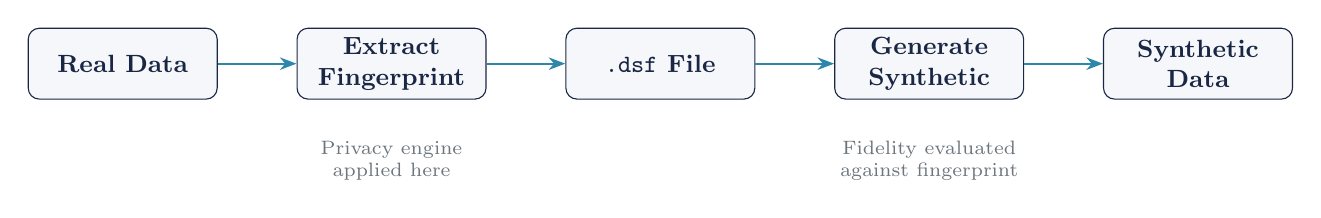
\begin{tikzpicture}[
  node distance=1.0cm,
  box/.style={draw=brand, fill=lightbg, rounded corners=4pt,
              minimum width=2.4cm, minimum height=0.9cm,
              font=\small\bfseries, text=brand, align=center},
  arr/.style={-{Stealth[length=6pt]}, thick, color=accent}
]
  \node[box] (real) {Real Data};
  \node[box, right=of real] (extract) {Extract\\Fingerprint};
  \node[box, right=of extract] (dsf) {\texttt{.dsf} File};
  \node[box, right=of dsf] (generate) {Generate\\Synthetic};
  \node[box, right=of generate] (output) {Synthetic\\Data};

  \draw[arr] (real) -- (extract);
  \draw[arr] (extract) -- (dsf);
  \draw[arr] (dsf) -- (generate);
  \draw[arr] (generate) -- (output);

  \node[below=0.4cm of extract, font=\scriptsize\color{midgray}, align=center]
    {Privacy engine\\applied here};
  \node[below=0.4cm of generate, font=\scriptsize\color{midgray}, align=center]
    {Fidelity evaluated\\against fingerprint};
\end{tikzpicture}
\end{center}

\subsection{Privacy Levels}

\begin{table}[h!]
\centering
\renewcommand{\arraystretch}{1.2}
\begin{tabularx}{\textwidth}{l c c c X}
\toprule
\textbf{Level} & \textbf{Epsilon ($\varepsilon$)} & \textbf{k-Anon} &
\textbf{Outlier \%} & \textbf{Use Case} \\
\midrule
Minimal  & 5.0  & 3  & 99\% & Low privacy, high utility \\
Standard & 1.0  & 5  & 95\% & Balanced (default) \\
High     & 0.5  & 10 & 90\% & Sensitive environments \\
Maximum  & 0.1  & 20 & 85\% & Maximum privacy guarantees \\
\bottomrule
\end{tabularx}
\end{table}

The privacy engine combines differential privacy (Laplace and Gaussian
mechanisms), k-anonymity with rare-value suppression, and outlier
winsorization. A full privacy audit trail records every decision and the
cumulative epsilon budget spent.

% ══════════════════════════════════════════════════════════════════════════════
\section{Architecture}

\subsection{Layered Crate Architecture}

\begin{center}
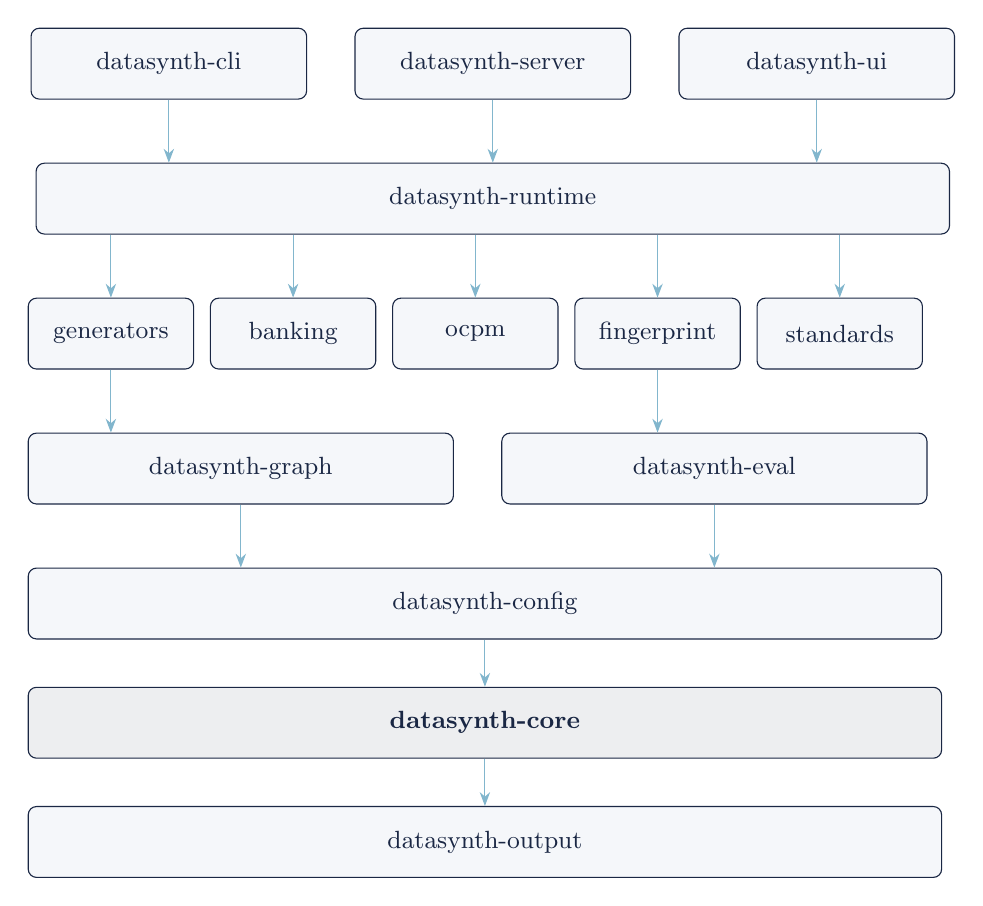
\begin{tikzpicture}[
  node distance=0.5cm,
  layer/.style={draw=brand, fill=lightbg, rounded corners=3pt,
                minimum height=0.9cm, font=\small, text=brand, align=center},
  arr/.style={-{Stealth[length=5pt]}, color=accent!60}
]
  % Top layer
  \node[layer, minimum width=3.5cm] (cli) {datasynth-cli};
  \node[layer, minimum width=3.5cm, right=0.6cm of cli] (server) {datasynth-server};
  \node[layer, minimum width=3.5cm, right=0.6cm of server] (ui) {datasynth-ui};

  % Runtime
  \node[layer, minimum width=11.6cm, below=0.8cm of server] (runtime) {datasynth-runtime};

  % Generator layer
  \node[layer, minimum width=2.1cm, below=0.8cm of runtime.south west,
        anchor=north west, xshift=-0.1cm] (gen) {generators};
  \node[layer, minimum width=2.1cm, right=0.2cm of gen] (bank) {banking};
  \node[layer, minimum width=2.1cm, right=0.2cm of bank] (ocpm) {ocpm};
  \node[layer, minimum width=2.1cm, right=0.2cm of ocpm] (fp) {fingerprint};
  \node[layer, minimum width=2.1cm, right=0.2cm of fp] (std) {standards};

  % Analytics layer
  \node[layer, minimum width=5.4cm, below=0.8cm of gen.south west,
        anchor=north west] (graph) {datasynth-graph};
  \node[layer, minimum width=5.4cm, right=0.6cm of graph] (eval) {datasynth-eval};

  % Config
  \node[layer, minimum width=11.6cm, below=0.8cm of graph.south west,
        anchor=north west] (config) {datasynth-config};

  % Core
  \node[layer, minimum width=11.6cm, below=0.6cm of config, fill=brand!8]
    (core) {\textbf{datasynth-core}};

  % Output
  \node[layer, minimum width=11.6cm, below=0.6cm of core] (output) {datasynth-output};

  % Arrows -- top to runtime (straight down from each)
  \draw[arr] (cli.south) -- (cli.south |- runtime.north);
  \draw[arr] (server.south) -- (runtime.north);
  \draw[arr] (ui.south) -- (ui.south |- runtime.north);

  % Runtime to generators (individual vertical drops)
  \draw[arr] (runtime.south -| gen) -- (gen.north);
  \draw[arr] (runtime.south -| bank) -- (bank.north);
  \draw[arr] (runtime.south -| ocpm) -- (ocpm.north);
  \draw[arr] (runtime.south -| fp) -- (fp.north);
  \draw[arr] (runtime.south -| std) -- (std.north);

  % Generators to analytics
  \draw[arr] (gen.south) -- (gen.south |- graph.north);
  \draw[arr] (fp.south) -- (fp.south |- eval.north);

  % Analytics to config
  \draw[arr] (graph.south) -- (graph.south |- config.north);
  \draw[arr] (eval.south) -- (eval.south |- config.north);

  \draw[arr] (config.south) -- (core.north);
  \draw[arr] (core.south) -- (output.north);
\end{tikzpicture}
\end{center}

\subsection{Production-Grade Infrastructure}

\begin{table}[h!]
\centering
\renewcommand{\arraystretch}{1.2}
\begin{tabularx}{\textwidth}{>{\bfseries\color{brand}}l X}
\toprule
\textbf{Capability} & \textbf{Details} \\
\midrule
Deterministic Output &
  ChaCha8 PRNG with configurable seed; identical seed $\Rightarrow$ identical
  dataset. \\
Financial Precision &
  \texttt{rust\_decimal} throughout; no IEEE\,754 floating-point artifacts.
  Decimals serialized as strings. \\
Resource Guards &
  Unified CPU, memory, and disk monitoring with automatic throttling and
  graceful degradation (Normal\,$\to$\,Reduced\,$\to$\,Minimal\,$\to$\,Emergency). \\
Collision-Free IDs &
  FNV-1a hash-based UUID factory with generator-type discriminators prevents
  document ID collisions across parallel generators. \\
API Layer &
  REST + gRPC + WebSocket with API-key authentication, sliding-window rate
  limiting, and configurable timeouts. \\
Desktop UI &
  Tauri + SvelteKit cross-platform application with 15+ configuration pages
  and real-time streaming viewer. \\
Python Wrapper &
  \texttt{datasynth-py} package with blueprints, pandas integration, and
  WebSocket streaming support. \\
\bottomrule
\end{tabularx}
\end{table}

% ══════════════════════════════════════════════════════════════════════════════
\newpage
\section{Industry Presets}

DataSynth ships with ten industry-specific configuration presets, each tuned
for realistic business process weightings, chart-of-accounts structures, and
regional multi-company setups.

\begin{table}[h!]
\centering
\renewcommand{\arraystretch}{1.25}
\begin{tabularx}{\textwidth}{>{\bfseries}l l X}
\toprule
\textbf{Industry} & \textbf{Key Weight} & \textbf{Characteristics} \\
\midrule
Manufacturing       & 40\% P2P & Heavy procurement, BOM-driven materials,
                                  multi-plant operations. \\
Retail              & 50\% O2C & High-volume sales, inventory-intensive,
                                  multi-currency. \\
Financial Services  & 40\% R2R & Report-heavy, regulatory compliance,
                                  intercompany structures. \\
Healthcare          & 15\% H2R & Labour-intensive, complex billing,
                                  compliance-driven. \\
Technology          & 15\% H2R & Knowledge workers, SaaS revenue recognition,
                                  R\&D capitalization. \\
Professional Svcs.  & --- & Time-based billing, project accounting. \\
Energy              & --- & Capital-intensive, long-lived assets. \\
Transportation      & --- & Fleet management, route-based costing. \\
Real Estate         & --- & Property portfolios, lease accounting. \\
Telecommunications  & --- & Subscription revenue, network assets. \\
\bottomrule
\end{tabularx}
\end{table}

Each preset supports three complexity tiers:
\textbf{Small} ($\sim$100 GL accounts),
\textbf{Medium} ($\sim$400 accounts), and
\textbf{Large} ($\sim$2\,500 accounts).

% ══════════════════════════════════════════════════════════════════════════════
\section{Use Cases}

\begin{tcolorbox}[keybox={Primary Use Cases}]
\begin{description}[leftmargin=1em, labelwidth=1em, font=\color{brand}\bfseries]
  \item[$\blacktriangleright$] \textbf{Fraud Detection ML} ---
    Train and validate models on labeled fraud typologies with realistic
    base-rate imbalance.

  \item[$\blacktriangleright$] \textbf{Graph Neural Networks} ---
    Export transaction graphs in PyTorch Geometric, Neo4j, or DGL format
    with pre-computed features and train/val/test splits.

  \item[$\blacktriangleright$] \textbf{AML \& KYC Testing} ---
    Generate banking transaction data with structuring, layering, and mule
    patterns for compliance system validation.

  \item[$\blacktriangleright$] \textbf{Audit Analytics} ---
    Produce ISA-compliant audit artifacts and anomaly-injected financial
    data for analytics tool development.

  \item[$\blacktriangleright$] \textbf{ERP Integration Testing} ---
    Generate SAP ACDOCA-format data with full document chains for system
    migration and integration testing.

  \item[$\blacktriangleright$] \textbf{Process Mining} ---
    OCEL\,2.0 event logs for process discovery, conformance checking, and
    variant analysis.

  \item[$\blacktriangleright$] \textbf{SOX \& COSO Compliance Testing} ---
    Internal control definitions with COSO 2013 mappings, SOX 302/404
    certifications, deficiency classification, and SoD conflict detection.

  \item[$\blacktriangleright$] \textbf{Accounting Standards Testing} ---
    Generate revenue contracts (ASC 606/IFRS 15), lease portfolios
    (ASC 842/IFRS 16), fair value measurements, and impairment tests
    with dual-framework reconciliation.

  \item[$\blacktriangleright$] \textbf{Data Quality ML} ---
    Labeled missing values, typos, duplicates, and format variations for
    training data-cleansing models.
\end{description}
\end{tcolorbox}

% ══════════════════════════════════════════════════════════════════════════════
\section{Evaluation \& Auto-Tuning}

DataSynth includes a built-in evaluation framework that measures synthetic
data quality across four dimensions:

\begin{enumerate}[leftmargin=1.4em, itemsep=3pt]
  \item \textbf{Statistical Fidelity} --- KS statistic, Wasserstein distance,
        Benford's Law MAD, amount distribution fit.
  \item \textbf{Coherence} --- Balance-sheet validation, intercompany matching,
        document chain integrity, subledger reconciliation.
  \item \textbf{Data Quality} --- Completeness, consistency, duplicate rates,
        format correctness, uniqueness.
  \item \textbf{ML Readiness} --- Feature distributions, label quality, graph
        structure, train/val/test split balance.
\end{enumerate}

An \textbf{auto-tuning engine} analyses evaluation results and produces
prioritized configuration patches with expected improvement estimates ---
closing the loop between generation and validation.

% ══════════════════════════════════════════════════════════════════════════════
\section{Getting Started}

\subsection{Quick Start (CLI)}

\begin{tcolorbox}[colback=brand!3, colframe=brand!40, boxrule=0.5pt, arc=3pt,
                   left=8pt, right=8pt, top=6pt, bottom=6pt]
\ttfamily\small
\# Generate with demo preset\\
datasynth-data generate --demo --output ./output\\[6pt]
\# Create an industry-specific config\\
datasynth-data init --industry manufacturing --complexity medium -o config.yaml\\[6pt]
\# Generate from config\\
datasynth-data generate --config config.yaml --output ./output
\end{tcolorbox}

\subsection{Quick Start (Python)}

\begin{tcolorbox}[colback=brand!3, colframe=brand!40, boxrule=0.5pt, arc=3pt,
                   left=8pt, right=8pt, top=6pt, bottom=6pt]
\ttfamily\small
from datasynth\_py import DataSynth\\
from datasynth\_py.config import blueprints\\[6pt]
config = blueprints.retail\_small(companies=4, transactions=10000)\\
synth = DataSynth()\\
result = synth.generate(config=config)
\end{tcolorbox}

\subsection{Server Mode}

\begin{tcolorbox}[colback=brand!3, colframe=brand!40, boxrule=0.5pt, arc=3pt,
                   left=8pt, right=8pt, top=6pt, bottom=6pt]
\ttfamily\small
\# Start REST/gRPC server with 4 worker threads\\
cargo run -p datasynth-server -- --port 3000 --worker-threads 4
\end{tcolorbox}

% ══════════════════════════════════════════════════════════════════════════════
\vspace{1.5em}
\begin{tcolorbox}[keybox={Links \& Resources}]
\renewcommand{\arraystretch}{1.4}
\begin{tabularx}{\textwidth}{>{\bfseries\color{brand}}l X}
  Repository &
    \url{https://github.com/ey-asu-rnd/SyntheticData} \\
  Documentation &
    \url{https://ey-asu-rnd.github.io/SyntheticData/} \\
  Crates.io &
    \url{https://crates.io/crates/datasynth-core} \\
  PyPI &
    \url{https://pypi.org/project/datasynth-py/} \\
\end{tabularx}
\end{tcolorbox}

\vfill
\begin{center}
\textcolor{midgray}{\rule{0.5\textwidth}{0.4pt}}\\[0.8em]
{\small\textcolor{midgray}{%
  DataSynth v0.2.3 \textbullet{}
  Open-source (Apache-2.0) \textbullet{}
  Commercial license available%
}}\\[4pt]
{\small\textcolor{midgray}{%
  \textbf{Contact:} \href{mailto:michael.ivertowski@ch.ey.com}{michael.ivertowski@ch.ey.com}%
}}
\end{center}

\end{document}
